\chapter{Arquitectura de la solución}

En este capítulo se describe detalladamente tanto la arquitectura de la aplicación, justificando cómo se cumplen los requisitos mencionados en la introducción, como la implementación propiamente dicha de cada uno de los elementos. También se incluye un caso de uso con un algoritmo concreto: Raft\cite{10.5555/2643634.2643666}.

\section{Análisis del problema}

Como se ha mencionado anteriormente, se desea visualizar una ejecución real del algoritmo, esto implica que debe existir algún medio de comunicación entre la interfaz y los nodos del mismo. Por tanto, es necesario que la aplicación que contiene la interfaz contenga además algún recurso capaz de interceptar o capturar los mensajes que se envían los nodos durante la ejecución del algoritmo. Este proceso \textit{manager} tiene como objetivo modificar la visualización en pantalla en base a los eventos que detecta en los nodos. Existen diversas alternativas para conseguir que reciba informacion en tiempo real de los mensajes de los nodos.

\section{Arquitectura de la interacción}
\label{sec:arquitectura}

La solución más sencilla a este problema consiste en modificar la funcionalidad del algoritmo que se ejecuta en los nodos, de tal forma que durante los envíos de mensajes se envíe también una copia al proceso \textit{manager}. En este caso el proceso \textit{manager} sería un simple servidor que recibe mensajes de los clientes (nodos del algoritmo) y actualiza la interfaz para representar los cambios de estado. Con esto sería necesario modificar ligeramente el algoritmo que se quiere visualizar. La arquitectura de esta solución se muestra en la Figura~\ref{fig:arquitectura1}

\newpage

\begin{figure}[h]
  \centering
  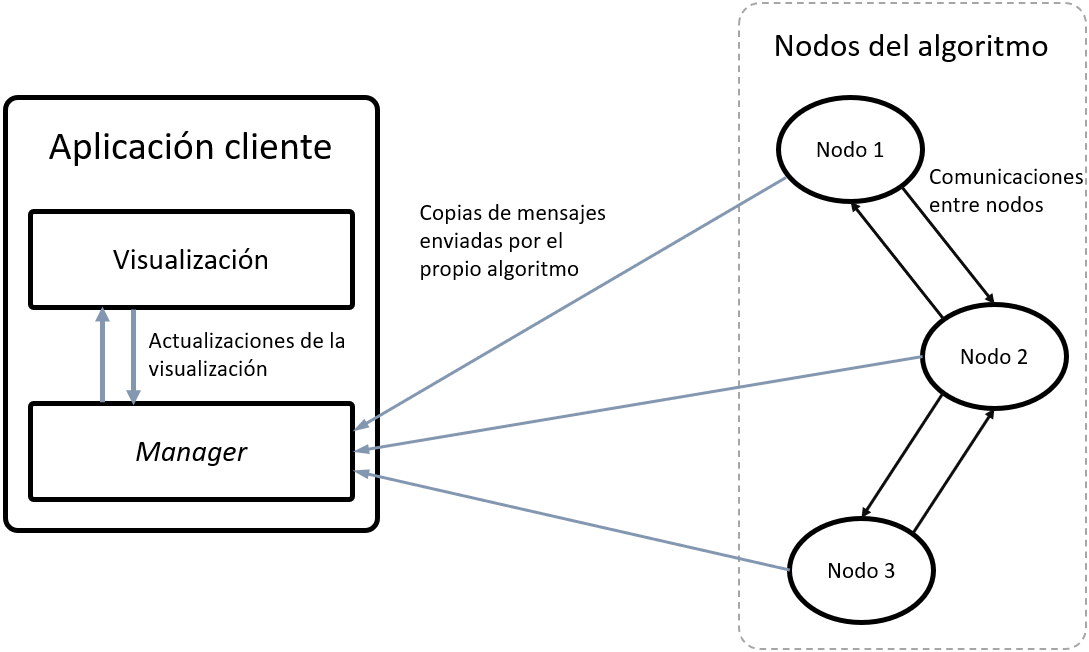
\includegraphics[width=0.7\linewidth]{imagenes/arquitectura1}
  \caption{Diagrama de la primera arquitectura propuesta}
  \label{fig:arquitectura1}
\end{figure}

En la Figura~\ref{fig:arquitectura1} se puede ver en la parte izquierda la aplicación cliente, que se compone de la interfaz, y del proceso \textit{manager} que la actualiza. Ambas partes se ejecutan en la misma máquina. En la parte de la derecha se localizan los nodos del algoritmo, que pueden ejecutarse en un entorno distribuido. Las flechas entre nodos simbolizan las comunicaciones del algoritmo, y las flechas entre cada nodo y el proceso \textit{manager} las copias de los mensajes.

Otra alternativa menos ``intrusiva`` en el algoritmo consiste en modificar de alguna manera las librerías que gestionan los envíos de paquetes de red. De tal forma que el algoritmo llama a la función de librería de envío de mensajes (\texttt{send}, \texttt{sendto}, \texttt{write}, etc) y esta envía una copia del mensaje al proceso \textit{manager}. Esta solución permite no tener que modificar nada del algoritmo. La arquitectura (Figura~\ref{fig:arquitectura2}) es muy parecida a la propuesta anteriormente, lo único que cambia es el origen del envío de las copias de mensajes.

\begin{figure}[h]
  \centering
  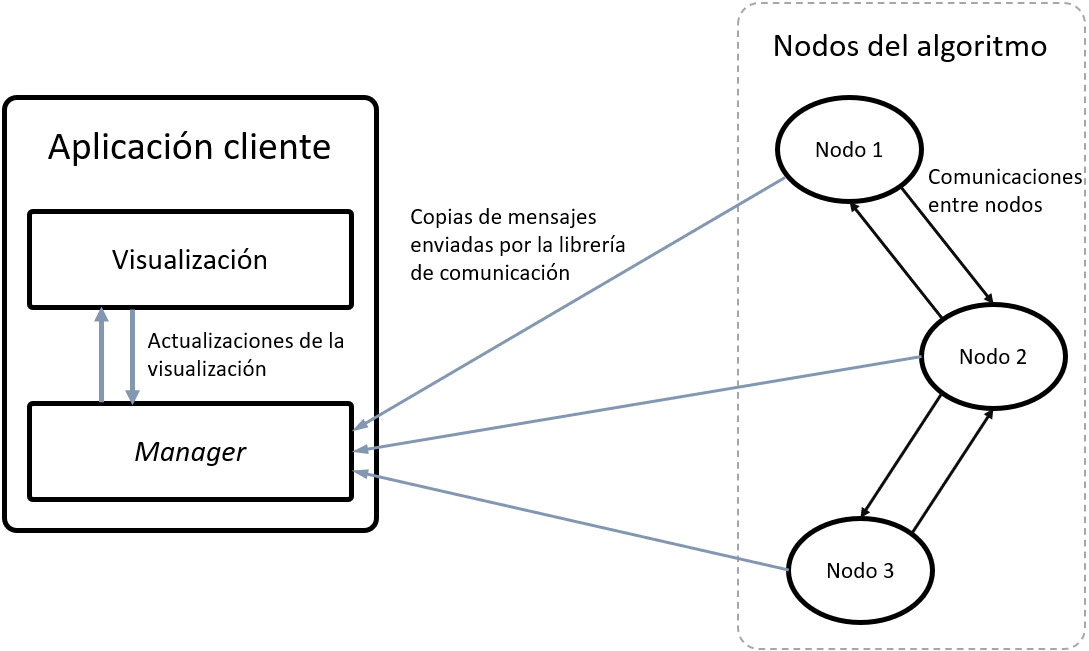
\includegraphics[width=0.7\linewidth]{imagenes/arquitectura2}
  \caption{Diagrama de la segunda arquitectura propuesta}
  \label{fig:arquitectura2}
\end{figure}

\newpage

Sin embargo esta alternativa cuenta con el gran defecto de que no sería posible intercambiar el algoritmo por otro implementado en otro lenguaje de programación cualquiera. Sería necesario volver a modificar las librerías necesarias. Esta resticción, junto con el hecho de que puede ser complicado modificar la funcionalidad incluída en las librerías del lenguaje, motiva la siguiente alternativa.

La alternativa final cuenta con otro proceso capturador o \textit{sniffer} que intercepta el tráfico de red a nivel de protocolo de un determinado proceso. Se ejecuta una instancia junto con cada nodo del algororitmo de tal forma que los mensajes capturados se reenvían al proceso \textit{manager} para que este actualize la visualización. Esta captura de mensajes se lleva a cabo a nivel de protocolo, por lo que no es necesario modificar ningún aspecto del algoritmo que se quiere visualizar. En esta solución el cuadro de mandos se abstrae totalmente del algoritmo, de forma que permite visualizar implementaciones en distrintos lenguajes, siempre que el medio de comunicación sea un protocolo conocido, por ejemplo TCP. Esta modificación se puede observar en la figura~\ref{fig:arquitectura3}.

\begin{figure}[h]
  \centering
  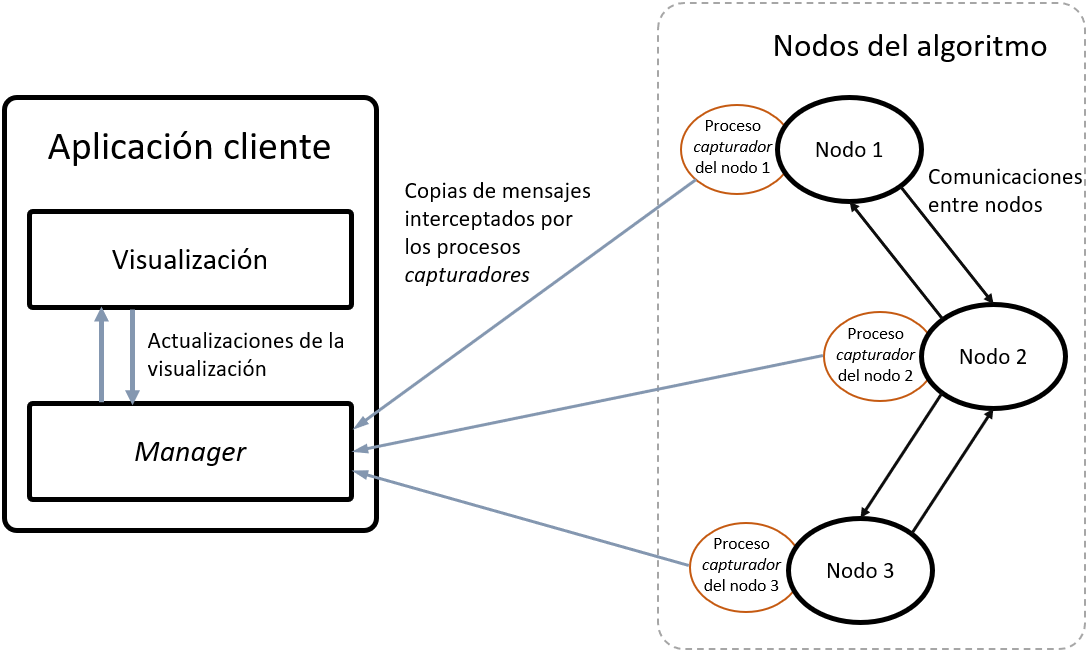
\includegraphics[width=0.7\linewidth]{imagenes/arquitectura3}
  \caption{Diagrama de la tercera arquitectura propuesta}
  \label{fig:arquitectura3}
\end{figure}

Por parte del proceso \textit{manager}, el funcionamiento es el mismo que en las soluciones propuestas anteriormente. Otra ventaja de esta arquitectura es que soportaría también visualizar algoritmos cuyo medio de comunicación se basa en las llamadas a procedimientos remotos (RPC). En las soluciones propuestas anteriores únicamente se tienen en cuenta los algoritmos cuyo modelo de comunicación se basa en el envío de mensajes entre \textit{sockets} (sería necesario modificar el proceso \textit{manger} para admitir la comunicación mediante RPC). Sin embargo, dado que las librerías de llamadas a procedimientos remotos también se basan en la comunicación con algún protocolo (por lo general TCP), también se capturarían estos mensajes.

La ventaja principal de esta arquitectura comparada con las anteriores, es que permite un desacoplamiento total del algoritmo. Además de esto, satisface los requisitos que se mencionan en la introducción.
